\documentclass{article}
\usepackage[utf8]{inputenc}

\title{Homework No.2}
\author{Osamu Katagiri-Tanaka : A01212611}
\date{\today}

% import math symbols
\usepackage{amsmath, esint}
\usepackage{cancel}

% import continuous lists
\usepackage{enumitem}

% format margins and paper size
\usepackage{geometry}
\geometry{
	paper         = a4paper, % Change to letterpaper for US letter
	inner         = 2.5cm,   % Inner margin
	outer         = 2.5cm,   % Outer margin
	bindingoffset = 0.5cm,   % Binding offset
	top           = 1.5cm,   % Top margin
	bottom        = 1.5cm    % Bottom margin
}

% import figure handler
\usepackage{graphicx}

\usepackage{longtable}

% import references handler
\usepackage[
    style     = ieee,         % references format style
    backend   = biber,        % choose the processing program
    natbib    = true,         % enable additional reference formats
    citestyle = numeric-comp, % enable multiple citations
    sortcites = true,         % sort references in multiple citations
    sorting   = nyt           % sort the reference table
]{biblatex}
\addbibresource{references.bib}

% Note that ‘d’ in the differential is conventionally set in roman.
\newcommand{\ud}{\,\mathrm{d}}

% Paragraph spacing
\setlength{\parskip}{0.2cm}           % spacing between paragraphs
\renewcommand{\baselinestretch}{1.25} % spacing between lines

\begin{document}

\maketitle

\section*{\emph{What will I achieve?}}
With this homework you will practice the use of the concepts and knowledge acquired throughout the corresponding topics.

\section*{Instructions}

\begin{enumerate}
\item \textit{Read \textbf{problem statement}, and collect the information that may be needed.}
\end{enumerate}

if the system initially is at $25^\circ C$, calculate:
\begin{itemize}
\item[a)] How long will it take to reach steady state (i.e. external heat is 98\% of the internal heat), and the heat rate as a function of time.
\item[b)] Temperature animation within the system for the first $24h$
\end{itemize}

\begin{enumerate}[resume]
\item \textit{Make a \textbf{Sketch} (Diagram, process flow chart), indicating mass, linear or angular momentum (i.e. forces and torques) and energy interaction, and label each stream and boundaries as well.}
\end{enumerate}

See Figure \ref{fig_SKETCH}

\begin{figure}[h!]
\centering
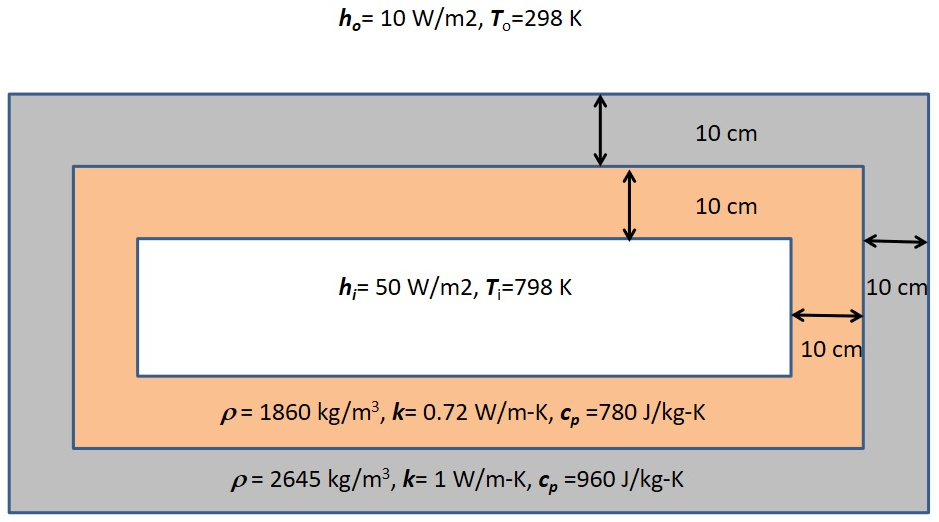
\includegraphics[width=0.75\textwidth]{./img/SKETCH.png}
\caption{Properties of a chimney: $4m$ long, $1m$ wide, and each wall in $10cm$ thick}
\label{fig_SKETCH}
\end{figure}

\begin{enumerate}[resume]
\item \textit{List \textbf{Assumptions and Approximations} (sometimes they may be inferred by the sketch, but make them explicit) supported by equations if possible (geometric relationships, or fundamental equations).}
\end{enumerate}

\begin{itemize}
\item The inner part heat transfer coefficient is $h_1 = 10 W/m^2$
\item The inner part heat transfer coefficient is $h_2 = 50 W/m^2$
\item The cold gas outside the chinmey is at a constant temperature $T_1 = 298 K$
\item The hot gas within the chimney is at a constant temperature $T_2 = 798.15 K$
\item the initial temperature of the system id $T_{init} = 298 K$
\item The "grey" wall is $2m$ long and $1m$ wide
\item The "orange" wall is $1.8m$ long and $0.8m$ wide
\item The "inner cavity" is $1.6m$ long and $0.6m$ wide
\end{itemize}

\begin{enumerate}[resume]
\item \textit{\textbf{Physical Laws} (Fundamental Laws) must be written in full form, and terms can be dropped by the right selection of frame of reference, operating conditions, assumptions, simplifications or constraints.}
\end{enumerate}

Parabolic PDE for heat transfer, as we are interested in the transient temperature

\begin{equation}
\rho c_P T' - div \left( \kappa grad(T) \right) = Q + h (T_{ext} - T)
\label{eq_heatTransfer}
\end{equation}

where: \\
$\rho$ is the density \\
$c_P$ is the heat capacity \\
$\kappa$ is the coefficient of heat conduction \\
$Q$ is the heat source \\
$h$ is the convective heat transfer coefficient \\
$T_ext$ is the external temperature 

\begin{enumerate}[resume]
\item \textit{\textbf{Physical constants} should be obtained from a reliable source (knowing this information by heart is always helpful ), geometric relations and formulae must be included as part of your analysis.}
\end{enumerate}

Not Applicable

%\begin{enumerate}[resume]
%\item \textit{\textbf{Physical transport or thermodynamic properties} (Thermodynamic relations) should be evaluated, approximated, calculated or obtained from a reliable source.}
%\end{enumerate}

\begin{enumerate}[resume]
\item \textit{\textbf{Calculations} are done including units. Any algebraic manipulation is recommended in few cases, because limits the step 8, but if needed should be done before using numerical values of constants, properties or variables.}
\end{enumerate}

% Set the x and y axes limits from -0.5 to 2.5 and from -0.5 to 1.5 respectively
% Show the grid to ease the drawing process
% Draw and edit the 2D geometry
%     Remove the chimney cavity by doing: (greyWall+orangeWall)-hotGas

As in Figure \ref{fig_drawing}, the first step is to draw the geometry of the chimney in the PDE tool in Matlab. The x and y axes limits are set to have a better view. In the "Set formula" field the following is specified: (greyWall+orangeWall)-hotGas. The "Set formula" value is to create the hotGas cavity of the chimney.

\begin{figure}[h!]
\centering
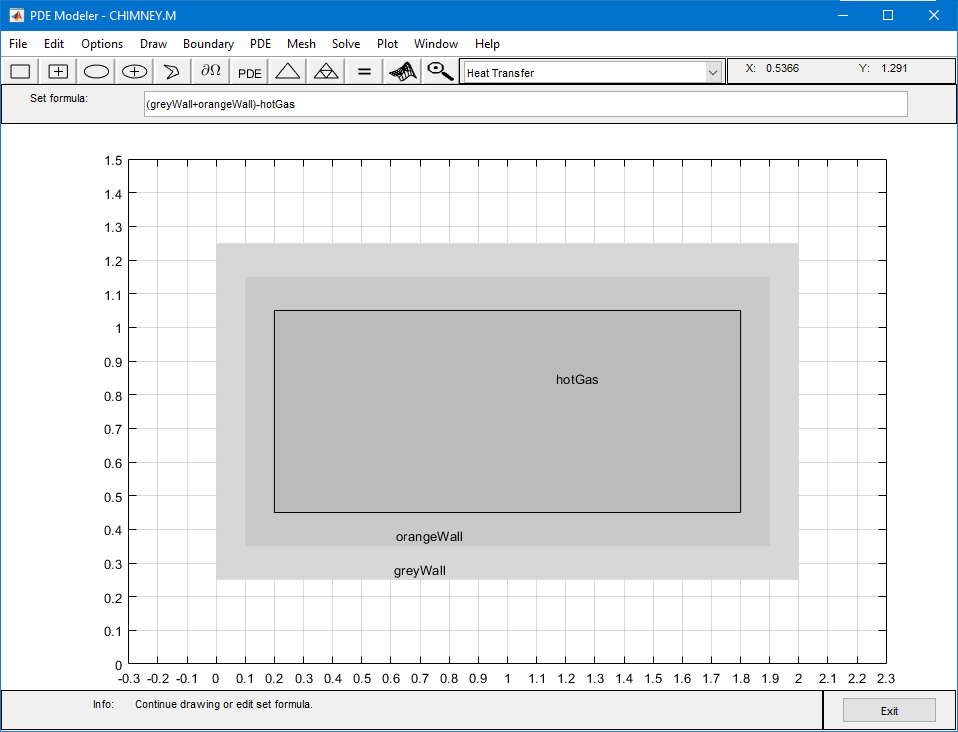
\includegraphics[width=0.70\textwidth]{./img/0_drawing.png}
\caption{Screen-shot of the drawing step}
\label{fig_drawing}
\end{figure}

% Discretize the geometry
The discretization result of the geometry is shown in Figure \ref{fig_discretizing}. This is done to show the correct use of  "Set formula" and the drawing process. A finer grid will yield better resolution results.

\begin{figure}[h!]
\centering
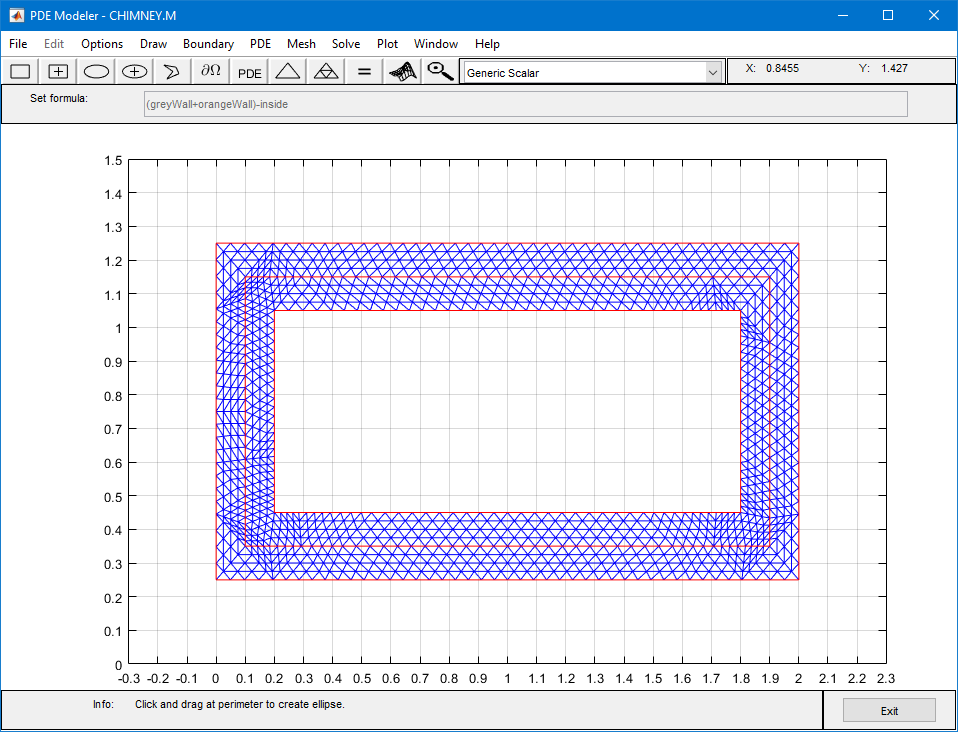
\includegraphics[width=0.70\textwidth]{./img/1_discretizing.png}
\caption{Screen-shot of the drawing step}
\label{fig_discretizing}
\end{figure}

% Specify the type of problem
Next step is to specify the type of problem of "Heat Transfer", as shown in Figure \ref{fig_specifyTheTypeOfProblem}.

\begin{figure}[h!]
\centering
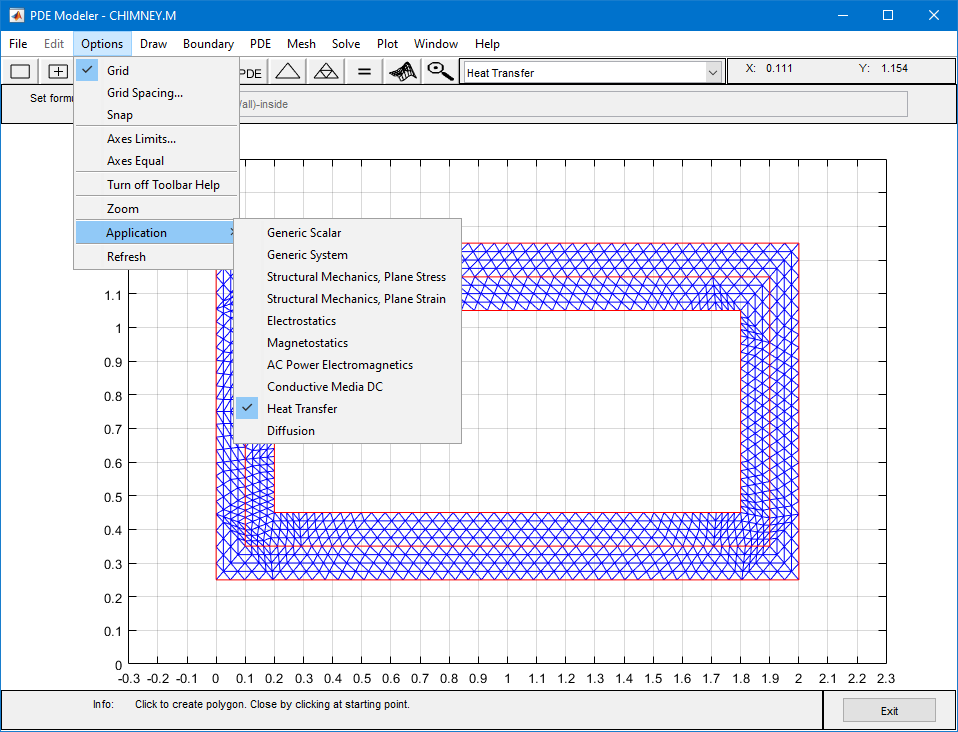
\includegraphics[width=0.70\textwidth]{./img/2_specifyTheTypeOfProblem.png}
\caption{Screen-shot of the drawing step}
\label{fig_specifyTheTypeOfProblem}
\end{figure} 

% Specify boundary conditions
Further, the boundary conditions shall be specified of type Neuman within the PDE tool. These conditions are set by the variables $g = q * T_{of}$ and $q$, the heat flux and the heat transfer coefficient respectively. $T_{of}$ is the temperature outside the boundary. See \ref{fig_specifyBoundaryConditions}.

\begin{figure}[h!]
\centering
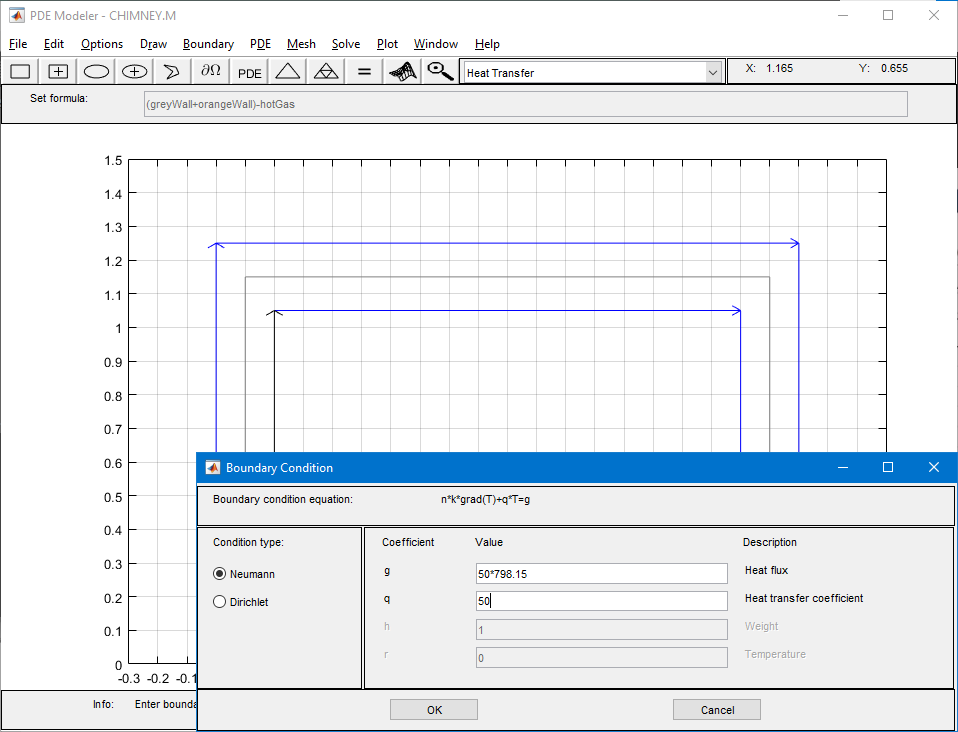
\includegraphics[width=0.70\textwidth]{./img/3_specifyBoundaryConditions.png}
\caption{Screen-shot of the drawing step}
\label{fig_specifyBoundaryConditions}
\end{figure}

% Specify the PDE type to describe the system
%    Elliptic is for steady state conditions
%    Parabolic is for transient conditions
On the other hand, the PDE of type parabolic is specified for each wall using Equation \ref{eq_heatTransfer}.

\begin{figure}[h!]
\centering
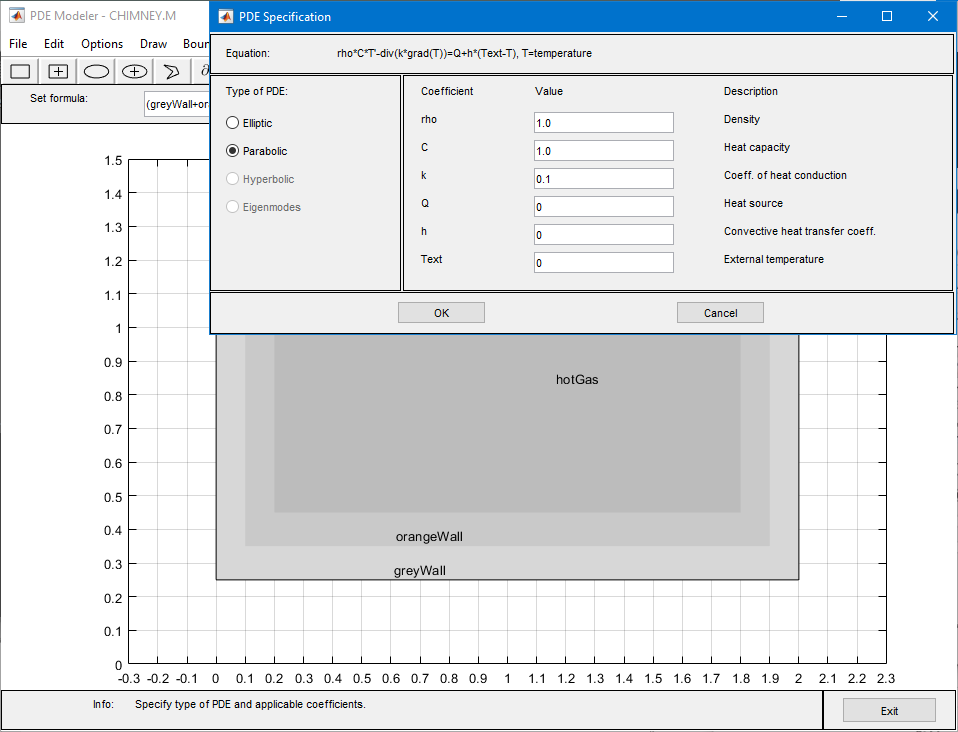
\includegraphics[width=0.70\textwidth]{./img/4_specifyThePDEtype.png}
\caption{Screen-shot of the drawing step}
\label{fig_SKETCH}
\end{figure}

% Solve PDE and run simulation

%\begin{figure}[h!]
%\centering
%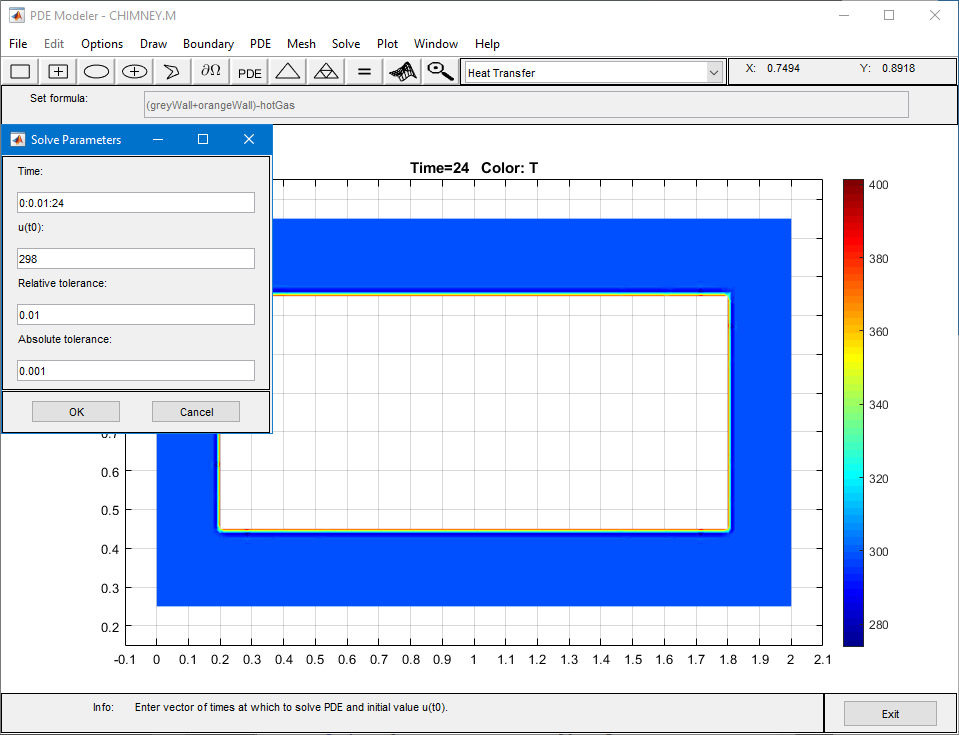
\includegraphics[width=0.70\textwidth]{./img/5_solvePDE.png}
%\caption{Screen-shot of the drawing step}
%\label{fig_SKETCH}
%\end{figure}

% Export the solution (transient temperature) and the mesh
% Calculate the Temperature at the walls T_W
% Calculate the Heat rate Q

Finally, the PDE solution is shown in Table \ref{tb_heatTransferAnimation} at different times. This solution assumes that the initial temperature of the system is of $298 K$

\begin{center}
\begin{longtable}{c  c}
    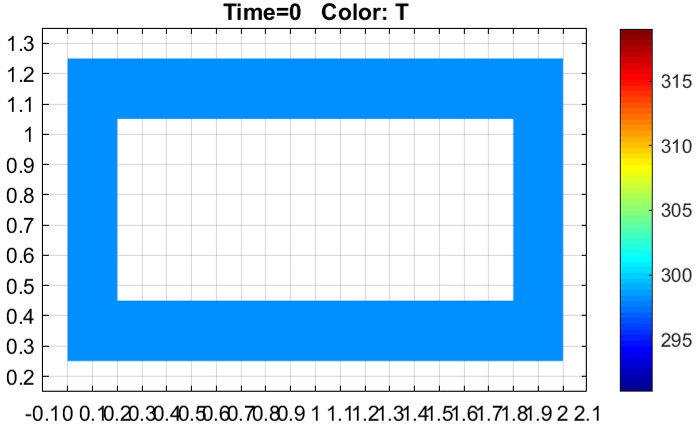
\includegraphics[width=0.5\textwidth]{./img/a00.png} &
    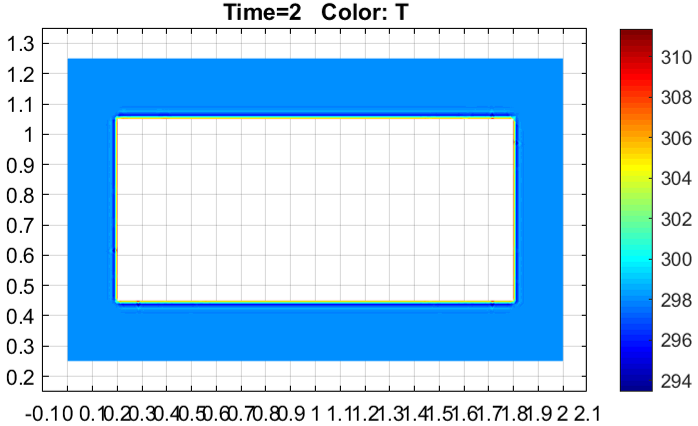
\includegraphics[width=0.5\textwidth]{./img/a02.png} \\
    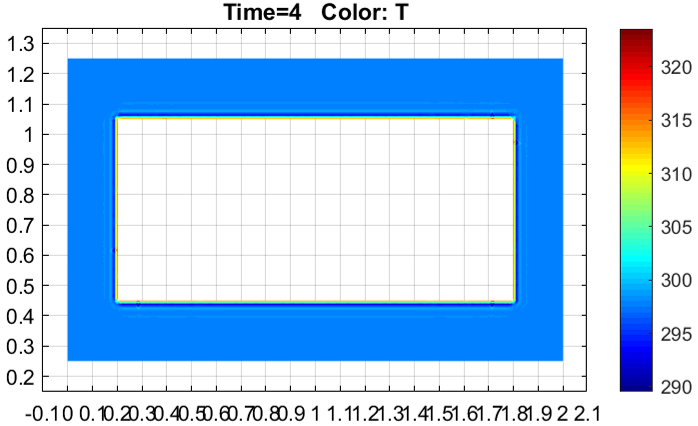
\includegraphics[width=0.5\textwidth]{./img/a04.png} &
    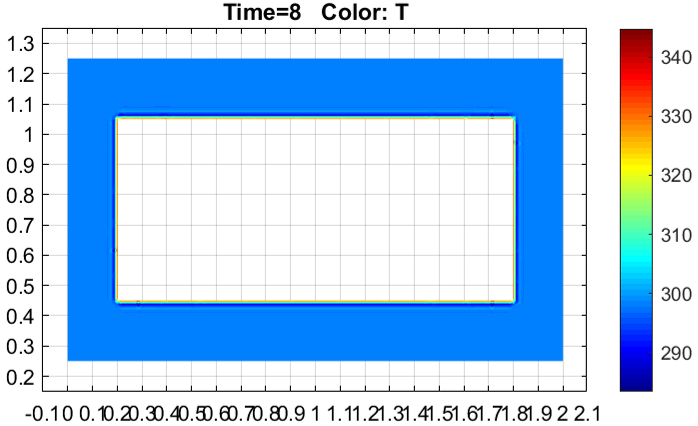
\includegraphics[width=0.5\textwidth]{./img/a08.png} \\
    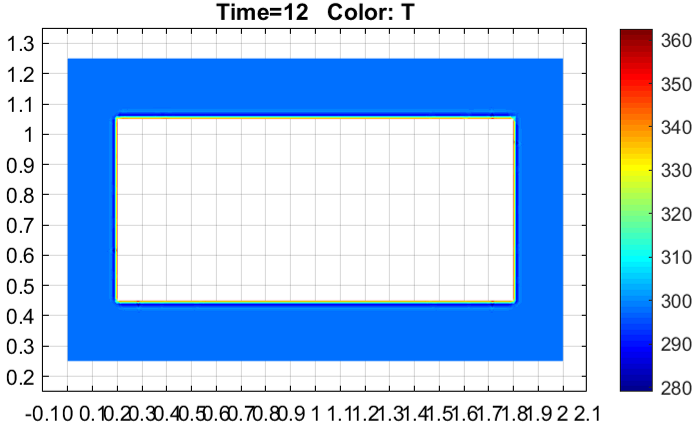
\includegraphics[width=0.5\textwidth]{./img/a12.png} &
    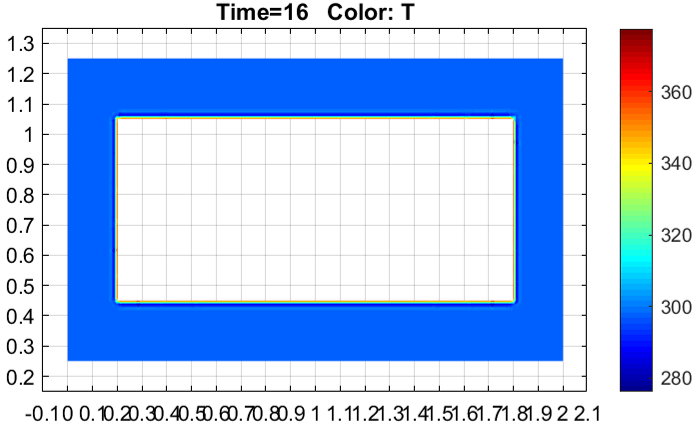
\includegraphics[width=0.5\textwidth]{./img/a16.png} \\
    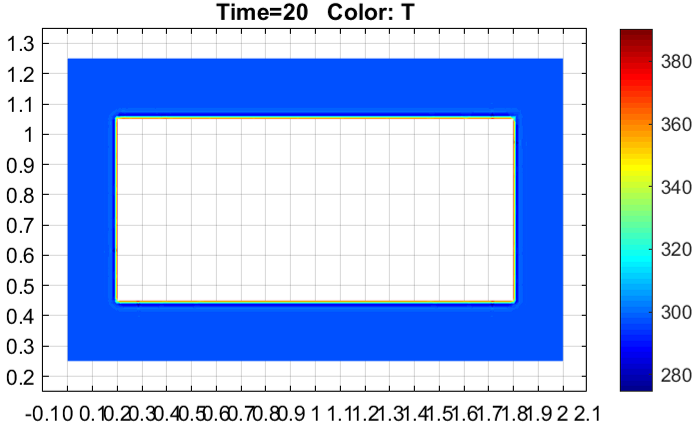
\includegraphics[width=0.5\textwidth]{./img/a20.png} &
    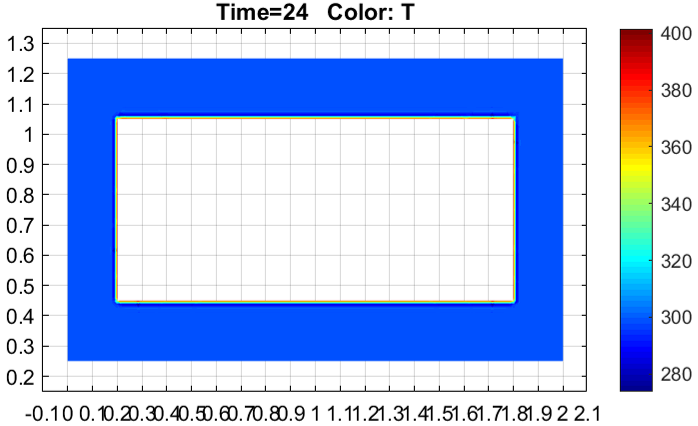
\includegraphics[width=0.5\textwidth]{./img/a24.png} \\
\caption{Heat transfer animation, where `Time' is in hours}
\label{tb_heatTransferAnimation}
\end{longtable}
\end{center}

%\begin{enumerate}[resume]
%\item \textit{\textbf{Reasoning} (Sensitivity analysis, what if), Verification (context), and Discussion should always be part of your answer to any problem, regardless the task requested.}
%\end{enumerate}

%\printbibliography[title={References}]
\end{document}